\documentclass[12pt]{article}

\usepackage{sbc-template}
\usepackage{graphicx,url}
\usepackage[T1]{fontenc}
\usepackage[utf8]{inputenc}
\usepackage[brazilian]{babel}
\usepackage{booktabs}
\usepackage{tabularx}
\usepackage{xcolor}
\usepackage[hidelinks]{hyperref}

\sloppy

\title{Synapse: Plataforma de Recomendação entre Profissionais e Projetos Internos com Arquitetura de Microsserviços e Apoio de Inteligência Artificial}

\author{Matheus Bachmann\inst{1}, Kauany Bloemer\inst{1}, Isaac Nilson Viana\inst{1}}

\address{Faculdade Donaduzzi\
Toledo -- Paraná -- Brasil
\email{matheusarthurbachmann@gmail.com, kauanybloemer04@gmail.com, isaacnilsonv@gmail.com}
}
\AddToHook{begindocument/before}[normalsf-fix]{\def\normalsfcodes{}}
\DeclareHookRule{begindocument/before}{normalsf-fix}{before}{babel}
\begin{document}

\maketitle

\begin{abstract}
  Internal mobility can help organizations use existing talent more effectively, but identifying suitable professionals for internal projects remains difficult when profile and opportunity information is fragmented or inconsistent. This paper presents Synapse, a functional web prototype that centralizes professional profiles, project portfolios, internal opportunities, expressions of interest, recommendations, and direct communication. The solution adopts a microservices architecture with a web frontend, an API gateway, domain services, separate databases, and a textual recommendation engine. Within the current scope, compatibility is calculated exclusively from the project description and from the professional's general and portfolio descriptions. Generative artificial intelligence assists users in improving these texts through questions and up to three reviewed reformulations, without automatic publication. The research follows a design science approach supported by a bibliographic study and iterative development. Functional validation covered containerized builds, service health checks, and integration flows through the API and interface. The prototype implements the intended end-to-end workflow, while the training and quantitative evaluation of the new description-based ranking model remain future work. Therefore, the current results concern the technical feasibility and functional integration of the platform, not the predictive quality of the recommendation model.
\end{abstract}

\begin{resumo}
  A mobilidade interna pode contribuir para que organizações aproveitem melhor os talentos já existentes, porém a identificação de profissionais adequados para projetos internos permanece difícil quando as informações de perfis e oportunidades estão fragmentadas ou são pouco descritivas. Este artigo apresenta a Synapse, um protótipo web funcional que centraliza perfis profissionais, portfólios de projetos, oportunidades internas, manifestações de interesse, recomendações e comunicação direta. A solução utiliza uma arquitetura de microsserviços composta por interface web, porta de entrada de APIs, serviços de domínio, bancos de dados separados e um motor de recomendação textual. No escopo atual, a compatibilidade considera exclusivamente a descrição da oportunidade e as descrições geral e de portfólio do profissional. A inteligência artificial generativa auxilia a qualificação desses textos por meio de perguntas e de até três reformulações revisáveis, sem publicação automática. A pesquisa segue uma abordagem de ciência do design, apoiada por pesquisa bibliográfica e desenvolvimento iterativo. A validação funcional incluiu compilação dos componentes em contêineres, verificação de saúde dos serviços e testes dos fluxos integrados pela API e pela interface. O protótipo implementa o fluxo principal proposto; o treinamento e a avaliação quantitativa do novo modelo de ordenação baseado em descrições permanecem como trabalho futuro. Assim, os resultados apresentados demonstram a viabilidade técnica e a integração funcional da plataforma, e não a qualidade preditiva do modelo de recomendação.

  \vspace{0.5cm}
  \noindent \textbf{Palavras-chave:} Mobilidade interna; Recomendação de profissionais; Inteligência artificial; Microsserviços; Descrições profissionais.
\end{resumo}

\section{Introdução}

A mobilidade interna corresponde ao movimento de pessoas entre funções, equipes ou níveis dentro de uma organização. Esse fenômeno abrange transferências e promoções e produz efeitos tanto para os indivíduos quanto para a organização \cite{ray2024internal}. Apesar de sua relevância, a descoberta de talentos internos ainda pode depender do conhecimento informal de gestores, de buscas manuais e de informações distribuídas em diferentes ferramentas. Nessas condições, profissionais com experiências adequadas podem não ser considerados para uma oportunidade simplesmente porque seu histórico não está visível ou suficientemente descrito.

Sistemas de recomendação pessoa--oportunidade procuram reduzir esse problema ao comparar informações de posições com informações profissionais. A literatura mostra que descrições de vagas e currículos podem ser tratadas como pares de textos para aprender relações semânticas e produzir ordenações de candidatos \cite{bian2019domain}. Entretanto, a aplicação dessa tecnologia em contextos de pessoas exige cautela. A pontuação deve apoiar a análise humana, e não substituir a decisão, pois opacidade, vieses nos dados e explicações insuficientes afetam a confiança e a justiça percebida \cite{tang2025explainable}.

Outro obstáculo prático é a qualidade do texto fornecido à plataforma. Descrições muito curtas, genéricas ou incompletas reduzem o contexto disponível para a recomendação. Por esse motivo, a solução desenvolvida combina dois usos distintos de inteligência artificial: um assistente generativo para ajudar a pessoa a tornar suas descrições mais objetivas e um motor responsável por ordenar perfis conforme a proximidade entre os textos. A reformulação é sempre apresentada para revisão, de modo que o usuário possa aceitá-la, editá-la ou solicitar uma nova rodada limitada.

\textcolor{blue}{O objetivo deste trabalho é desenvolver e integrar um protótipo funcional de plataforma para mobilidade interna, capaz de registrar perfis e projetos, qualificar descrições com apoio de modelos de linguagem e recomendar profissionais. No estado atual do protótipo, a ordenação utiliza provisoriamente um mecanismo determinístico de similaridade textual. A manifestação de interesse é apresentada apenas como um sinal complementar ao responsável pelo projeto, sem alterar a pontuação de compatibilidade ou a posição do profissional na ordenação. O treinamento e a avaliação quantitativa do modelo supervisionado de recomendação permanecem como trabalho futuro.}

O restante do artigo apresenta a fundamentação conceitual, descreve a metodologia adotada em narrativa contínua, detalha o protótipo implementado, discute os resultados funcionais e delimita as atividades que permanecem futuras.

\section{Fundamentação}

A mobilidade interna não é um processo uniforme: ela envolve objetivos da organização e expectativas individuais, podendo ocorrer horizontalmente, por transferências, ou verticalmente, por promoções \cite{ray2024internal}. Uma plataforma de oportunidades internas precisa, portanto, permitir participação ativa da pessoa. Na Synapse, essa participação ocorre tanto pela manutenção do perfil e do portfólio quanto pela possibilidade de demonstrar interesse em um projeto publicado.

Na recomendação pessoa--oportunidade, o conteúdo textual é uma fonte importante de evidência. Abordagens anteriores modelam a relação entre descrições profissionais e descrições de vagas como um problema de compatibilidade textual, inclusive em cenários com poucos exemplos rotulados \cite{bian2019domain}. No presente projeto, essa ideia fundamenta a decisão de usar apenas a descrição da oportunidade e a concatenação da apresentação profissional com as descrições dos projetos realizados. Campos isolados de habilidades, profissão e formação deixaram de compor a entrada do motor de recomendação, reduzindo a dependência de formulários rígidos e mantendo um contrato textual único.

Uma pontuação de compatibilidade não deve ser interpretada como probabilidade de contratação ou como avaliação definitiva de uma pessoa. Estudos sobre recomendação explicável ressaltam que sistemas aplicados a oportunidades de trabalho devem tornar claros os fatores usados e preservar supervisão humana \cite{tang2025explainable}. Consequentemente, a plataforma apresenta a pontuação como um indicador de proximidade textual. \textcolor{blue}{O interesse declarado é exibido separadamente como informação complementar e não modifica a pontuação ou a ordenação.} A decisão de aceitar, rejeitar ou reconsiderar um perfil permanece com o responsável pelo projeto.

A arquitetura de microsserviços organiza a aplicação em unidades implantáveis e alinhadas a responsabilidades específicas, mas também acrescenta custos de comunicação, operação e observabilidade \cite{pahl2016microservices}. Neste trabalho, a escolha foi mantida porque o protótipo é também uma atividade de integração entre componentes desenvolvidos por equipes distintas. A separação entre perfis, projetos, orquestração e inferência permite evoluir o contrato de recomendação sem acoplar o serviço de aprendizado de máquina aos bancos de negócio. Para uma implantação pequena, um monólito modular poderia atender ao mesmo fluxo com menor custo operacional; portanto, não se afirma que microsserviços sejam uma exigência universal do domínio.

\section{Metodologia}

O trabalho foi conduzido como pesquisa aplicada de ciência do design, abordagem voltada à construção e à avaliação de artefatos destinados a resolver problemas identificados \cite{peffers2007design}. A investigação partiu do problema de baixa visibilidade do talento interno e definiu como artefato um protótipo navegável capaz de integrar publicação de oportunidades, perfis profissionais e recomendação. Em apoio a essa construção, realizou-se uma pesquisa bibliográfica narrativa sobre mobilidade interna, recomendação pessoa--oportunidade, explicabilidade e arquitetura de microsserviços. As fontes foram selecionadas por pertinência ao problema, à construção do artefato e às limitações éticas discutidas no trabalho.

Com o problema e o escopo definidos, os requisitos foram registrados no repositório e transformados gradualmente em contratos de API, componentes de interface e serviços de domínio. O desenvolvimento seguiu ciclos curtos de implementação, integração e verificação, prática compatível com a evolução incremental de software descrita por \cite{pressman2021engenharia}. O ambiente foi padronizado com Docker Compose para que frontend, serviços, bancos PostgreSQL, cache Redis e motor de inferência pudessem ser iniciados de maneira reproduzível.

A entrada da recomendação foi delimitada a dois conteúdos: a descrição do projeto e a descrição consolidada do perfil, formada pela apresentação geral e pelos projetos de portfólio. Habilidades, ocupação, escolaridade e outros atributos estruturados não são enviados como variáveis independentes. O treinamento supervisionado do novo modelo textual foi separado da construção da plataforma e reservado para uma etapa posterior. Com isso, a avaliação descrita neste artigo permanece concentrada no funcionamento e na integração do artefato.

Paralelamente, foi implementado um assistente de escrita conectado, no servidor, aos provedores Gemini ou NVIDIA. O usuário fornece um texto inicial, responde a perguntas de esclarecimento e recebe uma reformulação. Cada sessão aceita no máximo três versões; as rodadas seguintes apresentam menos perguntas e uma nova sessão fica bloqueada por 24 horas. Nenhum texto é salvo automaticamente: a pessoa precisa aceitar ou editar o resultado. A mesma dinâmica é aplicada à descrição da oportunidade, à apresentação profissional e às descrições dos projetos do portfólio. \textcolor{blue}{O assistente recebe o tipo de contexto --- descrição de oportunidade, apresentação profissional ou projeto de portfólio ---, o texto atual e, na etapa de reformulação, as respostas fornecidas às perguntas de esclarecimento. Essas perguntas são geradas apenas para informações consideradas ausentes e procuram obter detalhes que tornem a descrição mais completa. As instruções enviadas ao modelo determinam que a reformulação seja clara, objetiva, inclusiva e fiel aos fatos informados, sem inventar tecnologias, resultados, experiências, salários ou responsabilidades. O texto gerado não substitui automaticamente o conteúdo original: ele é apresentado ao usuário, que pode aceitá-lo, editá-lo ou solicitar outra versão, respeitado o limite de três reformulações.}

\textcolor{blue}{A avaliação do artefato adotou como critérios a compilação dos componentes; a inicialização e a verificação de saúde dos onze contêineres; a comunicação entre a porta de entrada e os microsserviços; a persistência e a recuperação de dados; o funcionamento dos principais fluxos da plataforma; e a integração com o motor de recomendação. Esses critérios foram verificados por meio dos processos de compilação, das consultas aos indicadores de saúde, de requisições às APIs, da interação com a interface e dos testes automatizados disponíveis no motor de recomendação. A verificação utilizou contas e perfis de teste, sem coleta planejada de dados de trabalhadores para pesquisa.} Não foram conduzidos estudo com usuários, experimento controlado, comparação de algoritmos ou avaliação quantitativa do novo modelo textual. Essas limitações orientam a interpretação dos resultados apresentados neste artigo.

Embora a demonstração utilize dados de teste, uma implantação organizacional trataria informações pessoais e profissionais. Tal uso precisaria definir finalidade, base legal, controle de acesso, retenção e direitos dos titulares em conformidade com a Lei Geral de Proteção de Dados Pessoais \cite{brasil2018lgpd}. Também seriam necessárias avaliações de viés e mecanismos de contestação antes de empregar a recomendação em decisões reais.

\section{Desenvolvimento do Protótipo}

\subsection{Arquitetura e responsabilidades}

A Synapse é organizada como um monorrepositório e executada em contêineres. O frontend responsivo foi construído com Next.js e acessa o backend exclusivamente por uma porta de entrada de APIs. O \textit{Profile Service} mantém a apresentação profissional, a foto e o portfólio; o \textit{Project Service} concentra contas, projetos, manifestações de interesse, conversas, sessões do assistente generativo e telemetria; o \textit{Match Orchestrator} reúne os textos necessários e solicita as pontuações ao \textit{ML Engine}; e o \textit{ML Engine}, implementado com FastAPI, expõe a operação de inferência. Os dados de negócio são armazenados em bancos PostgreSQL separados por domínio, enquanto o Redis atua apenas como cache de perfis.

A autenticação utiliza um token de sessão enviado como credencial do tipo \textit{Bearer}. O cadastro público não exige que a pessoa escolha entre ``profissional'' e ``recrutador'': uma mesma conta pode manter seu perfil, publicar projetos e demonstrar interesse em projetos de outras pessoas. A propriedade do projeto é verificada no backend, o que impede tanto a alteração de projetos alheios quanto a manifestação de interesse no próprio projeto. O administrador permanece uma conta separada, provisionada por configuração do ambiente.

\subsection{Fluxos de uso}

O perfil profissional reúne apresentação geral e descrições dos projetos realizados. Ao criar uma oportunidade, o responsável informa título e descrição e pode usar o assistente generativo para obter um texto mais completo. Os projetos abertos aparecem em um feed central; cada cartão apresenta o responsável e a contagem agregada de interessados, sem revelar a identidade das demais pessoas. A visualização detalhada é aberta em uma janela sobre o feed e também permite registrar ou retirar o próprio interesse.

Quando o responsável consulta as recomendações de um projeto, o orquestrador combina a descrição da oportunidade com os textos de cada perfil e solicita uma pontuação de compatibilidade textual de zero a cem. O protótipo já possui o contrato e o fluxo de inferência da segunda versão, baseado exclusivamente em descrições. \textcolor{blue}{Enquanto o modelo supervisionado não é disponibilizado, o mecanismo provisório representa a descrição do projeto e a descrição consolidada de cada profissional por vetores TF--IDF e calcula entre eles a similaridade de cosseno. A pontuação textual é definida por}
\begin{equation}
\textcolor{blue}{S(p,c)=100 \times \cos\left(\mathbf{v}_{p},\mathbf{v}_{c}\right),}
\end{equation}
\textcolor{blue}{em que $\mathbf{v}_{p}$ representa o vetor da descrição do projeto e $\mathbf{v}_{c}$ representa o vetor formado pela apresentação geral e pelas descrições do portfólio do profissional. O resultado é limitado ao intervalo de zero a cem. A manifestação de interesse é exibida separadamente como informação complementar ao responsável pelo projeto, sem modificar a pontuação ou a posição do profissional na ordenação. Essa alternativa permite testar a integração, mas não substitui o treinamento nem sustenta conclusões sobre qualidade preditiva.}

A plataforma inclui ainda comunicação por chat, histórico de decisões sobre perfis, recuperação de senha por e-mail e um painel administrativo para acompanhar consumo e estimativas de custo dos tokens de entrada e saída usados pelo assistente generativo. As credenciais dos provedores de linguagem permanecem no backend e não são expostas ao navegador.

\section{Resultados e Discussão}

O resultado obtido é um protótipo integrado que executa o percurso principal desde a criação de uma conta até a análise de profissionais para um projeto. Na verificação realizada no ambiente local, os onze contêineres previstos permaneceram em execução; a porta de entrada respondeu com estado \texttt{UP} e confirmou o mesmo estado para os serviços de perfis, projetos e orquestração. Os dois testes automatizados disponíveis no motor de inferência também foram aprovados: um verifica se a descrição profissional textualmente mais próxima ocupa a primeira posição e o outro confirma o retorno de todos os perfis, inclusive quando uma descrição está vazia. A Tabela~\ref{tab:resultados} resume as entregas verificadas no estado atual do repositório.

\begin{table}[ht]
\centering
\caption{\textcolor{blue}{Evidências objetivas da verificação do protótipo.}}
\label{tab:verificacoes}
\begin{tabularx}{\textwidth}{p{0.25\textwidth}X X}
\toprule
\textcolor{blue}{\textbf{Verificação}} & \textcolor{blue}{\textbf{Resultado esperado}} & \textcolor{blue}{\textbf{Resultado observado}} \\
\midrule
\textcolor{blue}{Compilação dos componentes} & \textcolor{blue}{Concluir a construção sem erros} & \textcolor{blue}{Frontend, serviços Java e motor de recomendação compilados com sucesso} \\
\textcolor{blue}{Inicialização do ambiente} & \textcolor{blue}{Manter os onze contêineres em execução} & \textcolor{blue}{Onze contêineres iniciados; serviços monitorados apresentaram estado saudável} \\
\textcolor{blue}{Saúde das dependências} & \textcolor{blue}{Obter estado disponível para os serviços integrados} & \textcolor{blue}{Porta de entrada e serviços de perfis, projetos e orquestração responderam com estado \texttt{UP}} \\
\textcolor{blue}{Interface web} & \textcolor{blue}{Disponibilizar a aplicação no navegador} & \textcolor{blue}{Frontend respondeu com código HTTP 200} \\
\textcolor{blue}{Motor de recomendação} & \textcolor{blue}{Ordenar o perfil textualmente mais próximo e preservar candidatos sem descrição} & \textcolor{blue}{Dois testes automatizados executados e aprovados} \\
\bottomrule
\end{tabularx}
\end{table}

A Figura~\ref{fig:feed} registra o feed de oportunidades em execução. A captura evidencia a navegação unificada, a apresentação resumida do perfil, a identificação da pessoa responsável pelo projeto, a descrição da oportunidade, a contagem de interessados e o acesso à visualização detalhada.

\begin{figure}[ht]
\centering
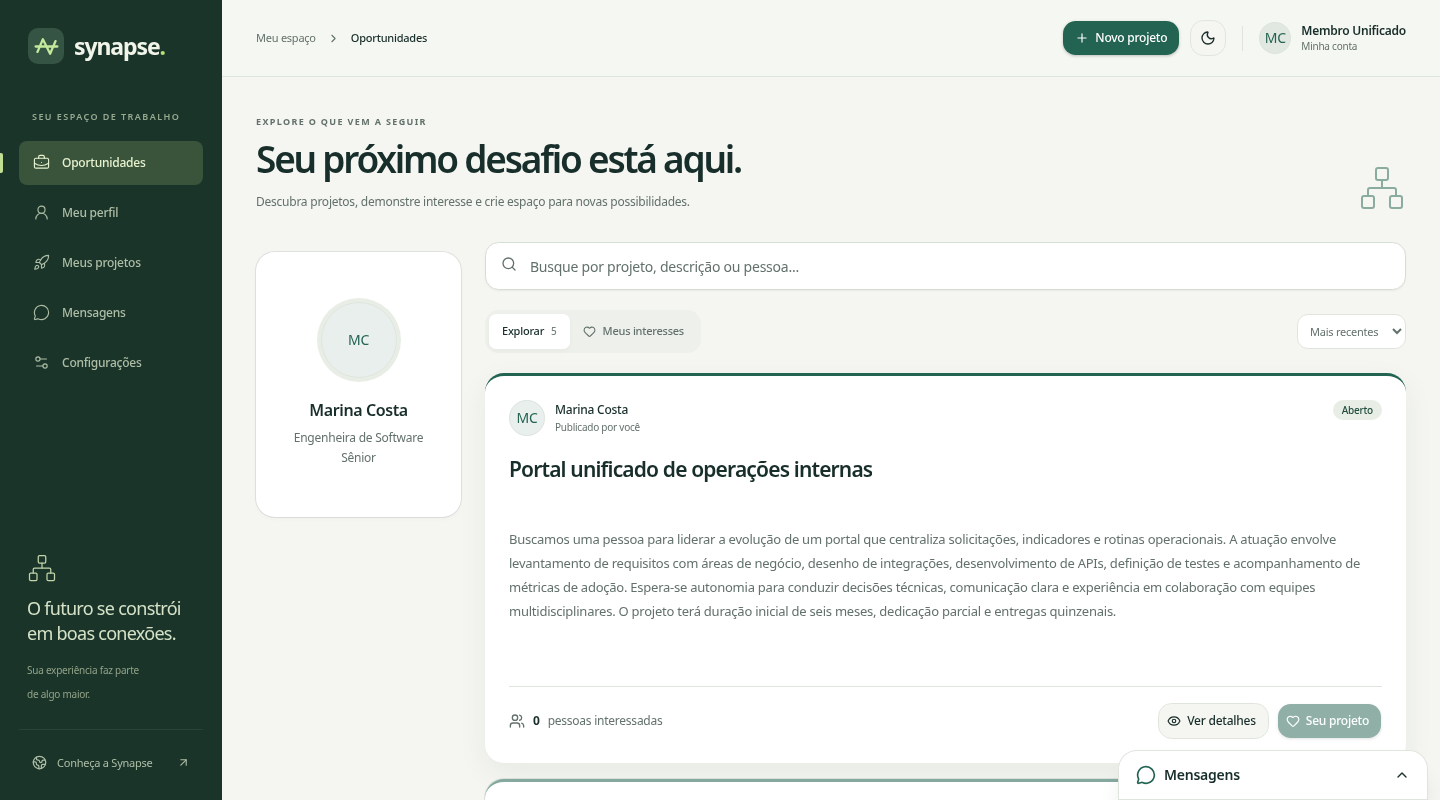
\includegraphics[width=\textwidth]{figuras/feed-synapse.png}
\caption{\textcolor{blue}{Feed de oportunidades do protótipo Synapse em execução.}}
\label{fig:feed}
\end{figure}

\begin{table}[ht]
\centering
\caption{\textcolor{blue}{Fluxos implementados e respectivas evidências funcionais.}}
\label{tab:resultados}
\begin{tabularx}{\textwidth}{p{0.19\textwidth}p{0.32\textwidth}X}
\toprule
\textcolor{blue}{\textbf{Fluxo}} & \textcolor{blue}{\textbf{Funcionalidade implementada}} & \textcolor{blue}{\textbf{Evidência funcional}} \\
\midrule
\textcolor{blue}{Conta e segurança} & \textcolor{blue}{Cadastro, autenticação, troca e recuperação de senha} & \textcolor{blue}{Fluxos executados com contas de teste e recuperação por link de uso único} \\
\textcolor{blue}{Perfil profissional} & \textcolor{blue}{Apresentação, foto e projetos de portfólio} & \textcolor{blue}{Dados salvos e recuperados pela interface e pelo serviço de perfis} \\
\textcolor{blue}{Projetos e feed} & \textcolor{blue}{Criação, edição, listagem e visualização de projetos} & \textcolor{blue}{Projetos persistidos e apresentados no feed, conforme registrado na Figura~\ref{fig:feed}} \\
\textcolor{blue}{Interesse} & \textcolor{blue}{Registro e retirada da manifestação de interesse} & \textcolor{blue}{Estado e contagem atualizados, com bloqueio de interesse no próprio projeto} \\
\textcolor{blue}{Recomendação} & \textcolor{blue}{Comparação textual e ordenação de profissionais} & \textcolor{blue}{Dois testes automatizados aprovados; interesse exibido sem alterar pontuação ou ordenação} \\
\textcolor{blue}{Comunicação} & \textcolor{blue}{Chat, mensagens não lidas e notas particulares} & \textcolor{blue}{Envio, recuperação e apresentação das mensagens verificados com contas de teste} \\
\textcolor{blue}{Assistente de escrita} & \textcolor{blue}{Perguntas, reformulações e revisão pelo usuário} & \textcolor{blue}{Limite de três versões e necessidade de aceite ou edição confirmados no fluxo} \\
\bottomrule
\end{tabularx}
\end{table}

Os testes funcionais confirmaram que os serviços podem ser construídos e iniciados de forma conjunta, que a porta de entrada encaminha as requisições aos domínios correspondentes e que os principais fluxos persistem e recuperam seus dados. A interface foi adaptada para computadores e dispositivos móveis e concentra o feed, o perfil resumido e o acesso rápido às conversas. Esses resultados respondem ao objetivo de demonstrar a viabilidade técnica da plataforma integrada.

A avaliação funcional não permite inferir a qualidade preditiva da recomendação. Para o contrato textual atual, ainda não foram obtidas métricas de ordenação nem realizada comparação entre algoritmos. O conjunto de dados a ser adotado também deverá conter pares de descrições e rótulos compatíveis com a tarefa definida. Por essa razão, os resultados ficam restritos ao comportamento observável do protótipo e à integração entre seus componentes.

O protótipo apresenta limitações. A atualização do chat utiliza consultas periódicas, as fotos ainda são armazenadas como dados textuais, e a avaliação realizada verifica funcionamento, não usabilidade ou impacto organizacional. Além disso, a compatibilidade textual pode reproduzir vieses presentes nas descrições e pode favorecer textos mais detalhados. O assistente generativo reduz parcialmente a diferença de qualidade textual, mas sua saída também precisa ser revisada pelo usuário. Essas limitações reforçam que a ferramenta oferece apoio à decisão e não uma decisão automática sobre pessoas.

\section{Considerações Finais}

Este trabalho apresentou a versão funcional da Synapse, uma plataforma de recomendação entre profissionais e projetos internos. O escopo foi concentrado na integração entre perfil, portfólio, projetos, feed de oportunidades, interesse, recomendação textual, assistência de escrita e comunicação. Essa delimitação permitiu substituir afirmações prospectivas por resultados observáveis no protótipo e esclarecer as fronteiras da contribuição.

A solução demonstra que é tecnicamente possível reunir descrições profissionais e de projetos em um fluxo único e produzir uma ordenação baseada na proximidade textual. \textcolor{blue}{O interesse voluntariamente manifestado é apresentado separadamente como informação complementar e não modifica a pontuação ou a ordenação.} A arquitetura distribuída separa as responsabilidades dos domínios e do motor de inferência, embora aumente a complexidade operacional e não seja apresentada como única solução possível.

Como continuidade, será necessário selecionar e documentar um conjunto de pares textuais compatível com o novo contrato, treinar o modelo baseado exclusivamente em descrições e avaliá-lo com métricas próprias de ordenação, como o ganho cumulativo descontado normalizado em uma posição de corte (NDCG@$k$) e a posição recíproca média (MRR). Também devem ser realizados testes com usuários, avaliação de vieses, análise de explicabilidade e comparação do protótipo com um processo manual. Somente após essas etapas será possível discutir a qualidade das recomendações e o impacto da plataforma na mobilidade interna.

\bibliographystyle{sbc}
\bibliography{sbc-template}

\end{document}
